 % !Mode:: "TeX:UTF-8"
\chapter{可见光多波段OFDM系统速率自适应技术研究}
\section{引言}
自适应传输技术在上世纪60年代就已经被提出,其基本思想就是根据实时的信道质量决定调制参数,目标是优化通信质量,但是因为其计算复杂度很大,实现困难而没有引起研究人员足够的重视\cite{徐凌峰2007ofdm},直到上世纪80年代末,人们对高速可靠的通信系统的需求越来越强烈,同时由于数字集成电路的快速发展,其计算能力已能够支撑复杂的算法,所以自适应传输计算重新进入研究人员的视野,并且成功用于DSL、WCDMA等通信系统。前面我们已经介绍过OFDM系统及其信道估计的方法,已经了解OFDM技术是把实际通信信道划分成若干个子信道,每个子信道可以认为是独立传输的,如果所有的子载波上都使用同样的调制方式,那么整个系统的误比特率性能就由那些处于深衰落处的子载波决定,如在前两章已经介绍室内可见光信道就是低通的,则此时高频的子载波决定了整个系统的性能,这样的方法显然是不合理的,所以在第三章的仿真中就使用了表\ref{tab:modOrder}所示的调制策略,但是之前得到这样的策略是由主观判断得到的,而没有充足的理论依据。本章将详细介绍OFDM自适应技术及其在可见光通信中的应用,首先将从信息论的角度探讨自适应传输的原理,然后将介绍现有的几种经典的自适应算法并且仿真分析它们的性能,最后将介绍一种可见光自适应传输方案。
\section{自适应传输的信息论基础}
通信技术经过将近一个世纪的发展,不断出现的使得系统传输速率越来越高,因此人们要问在特定的通信信道下传输速率的极限是什么?这正是经典的香农信息论已经回答的问题,同时也给系统设计者指明了要达到这个极限系统要满足的条件,虽然这些严苛的条件在实际设计中不可能完全满足,但是已有很多系统的系统已经很接近香农限了。

自适应传输是一种提高频谱利用率的通信技术,同样也满足香农信息论关于信道容量的结论,所以自适应传输技术也不可能使得实际系统传输速率突破香农限,而是在香农信息论的指导下去设计系统,使得系统逼近这一极限,因此在讨论自适应传输的具体算法之前了解一些香农信息论的知识非常必要。
\subsection{高斯信道容量}
信道容量是一个通信信道环境一个重要的度量指标,它的含义是在该信道下传输速率的上限,如果本身信道容量就很小的环境下,无论使用何种通信技术也不能实现高速通信系统,反之在信道容量大的信道环境下,可以通过精心设计系统以达到高速通信的目的。在香农信息论中,信道容量是用互信息量来描述的,其数学表达式为:
\begin{equation}
C = \arg \underset{P_x(X)}{\text{max}} \ I(X;Y)
\end{equation}

\begin{equation}
I(X;Y)=\sum_{x,y}p(x,y)\log_2\frac{p(x,y)}{p(x)p(y)}
\end{equation}
式中$I(X;Y)$表示发送信号X与接收信号Y之间的互信息,p(x)、p(y)和p(x,y)分别表示X=x的概率,Y=y的概率及X=x并且Y=y的联合概率。根据上面的定义,我们可以得到在高斯信道下的信道容量公式为:
\begin{equation}
C = B\log_2\left(1+\frac{S}{N_0B}\right)=B\log_2(1+\gamma)
\end{equation}
上式中B为高斯信道带宽,S为输入信号的平均功率,$N_0$为单边带高斯噪声功率谱密度,$\gamma=\frac{S}{N_0B}$表示接收信噪比。该容量是当发送信号X服从高斯分布时取得。而在实际的数字传输系统中,这个条件是无法满足的,所以该信道容量只能作为系统传输速率的上限。
\subsection{注水定理}
在无线通信环境下,由于放大器等硬件是非理想的,并且信号在传输过程中会发生散射、反射等造成多径,实际的通信系统信道远比加性高斯信道复杂得多。我们假设信道的传输函数为$H(f)$,输入信号的功率谱密度为$S(f)$,单边带高斯噪声功率密度还是$N_0$。为了推到这样的信道的信道容量,可见将整个信道带宽均分为N个子信道,则每个子信道的带宽为$B/N$,当N足够大时,中心频率为$f_i$处的子信道可以看作是信道增益为$H(f_i)$的带限信道。于是整个信道容量等于所以子信道容量之和:
\begin{equation}
\begin{aligned}
C&=\lim_{N\rightarrow \infty}\sum_{i=1}^{N}\Delta f\log_2\left(1+\frac{S(f)|H(f)|^2\Delta f}{N_0 \Delta f}\right) \\
&=\int_B \log_2\left(1+\frac{S(f)|H(f)|^2}{N_0}\right)df
\end{aligned}
\end{equation}
从上式中可以看出信道传输函数H(f)和发送信号的功率谱密度分布及噪声功率共同决定了信道容量的大小。假设系统发射功率受限,即:
\begin{equation}
\label{equ:powerLimit}
\int_B S(f)df=P
\end{equation}
则由拉格朗日乘子法计算可得,当S(f)的分布满足下式时可以达到信道容量。
\begin{equation}
\label{equ:water_filling}
S(f)=
\begin{aligned}
\begin{cases}
K-\frac{N_0}{|H(f)|^2},&\ |H(f)|^2\geq\frac{N_0}{K} \\
0  ,&\ |H(f)|^2<\frac{N_0}{K}
\end{cases}
\end{aligned}
\end{equation}
其中K为常数,并且满足式\ref{equ:powerLimit}中的功率受限条件。

式\ref{equ:water_filling}得到S(f)分布的过程也称为“注水定理”或者“注水算法”,它表示要想在传输函数为H(f),噪声功率密度为$N_0$的信道下要达到信道容量S(f)的分布一定要满足上式。其物理含义是:当信噪比$|H(f)|^2/N_0$较大时,应该给该处的子信道分配更多的功率;反之当信噪比很小时,分配的功率也很小;甚至当信噪比过小(小于1/K)时不分配功率。
\begin{figure}[htbp]
\centering
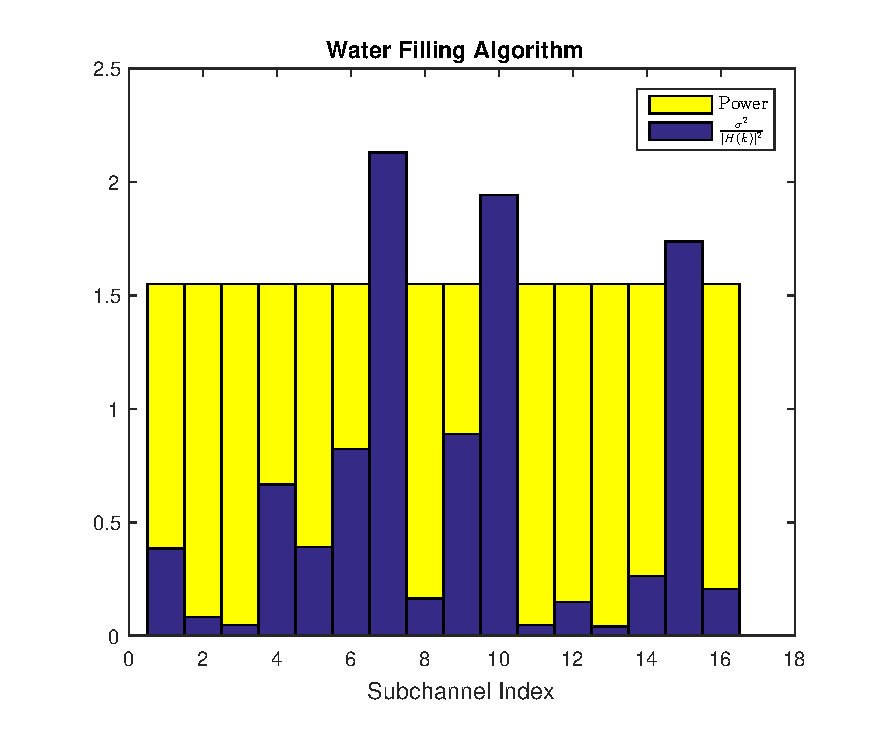
\includegraphics[width=0.9\textwidth]{figures/chapter-4/waterFilling.eps}
\caption{注水定理示意图}
\label{fig:waterFilling}
\end{figure}
OFDM技术的基本原理就是将整个信道划分为相互正交的并行子信道,这个与前面注水算法的推导过程很相识,只是OFDM系统中子载波的数目是有限的,调制阶数是离散的。从此可以看出注水算法很容易在OFDM系统中现实,我们将在下一节中详细介绍。
\section{OFDM系统自适应算法研究}
在一个有N个子载波的OFDM系统中,假设各个子载波上的信道增益$h_k=|H(k)|^2(k=0,1,\cdots,N-1)$和高斯噪声方差$\sigma^2$已知,若$b_k$和$p_k$分别表示分配到第k个子载波上比特数和功率,如设置误比特率为固定值$\text{BER}_{target}$,则香农公式$b_k$与$p_k$有如下关系:
\begin{equation}
b_k = \log_2(1+\frac{h_kp_k}{\Gamma\sigma^2})
\end{equation}
也可以写为:
\begin{equation}
p_k = \frac{\Gamma\sigma^2}{h_k}(2^{b_k}-1)
\end{equation}
其中$\Gamma$表示信噪比差(SNR gap),它由误比特率BER及调制星座图决定,对于QAM调制,如不加信道编码,则$\Gamma$与$\text{BER}_{target}$之间关系如下\cite{余官定2005ofdm}:
\begin{equation}
\Gamma = -\frac{\ln(5\cdot\text{BER}_{target})}{1.5}
\end{equation}

OFDM自适应传输在不考虑信道编码的情况下其实就是比特和功率在各个子载波上分配问题,它可以有传输速率、发射功率和误比特率三个优化目标量,这样也就有三种优化准则,即固定误比特率和功率的速率最大化(Rate Adaptive,RA)准则、固定误比特率和速率的功率最小化(Margin Adaptive, MA)准则和固定功率和速率的误比特率最小化(BER Adaptive, BA)准则。同时需要提出的是,与前面的理论分析不同,实际系统可以选择的调制方式是离散的($b_k \in \mathbb{N}$,$\mathbb{N}$表示整数集),也就是说OFDM自适应其实是一个整数优化问题(Integer Programming,IP),之前在推导注水算法时用到的拉格朗日乘子法不能再用到实际系统中,需要根据实际系统的需要,根据优化准则去选择合适的优化方法,下面将介绍几种经典的OFDM自适应算法。
\subsection{Hughes-Hartogs算法}
Hughes-Hartogs算\cite{hughes1989ensemble}法受数学中“贪婪(Greedy)优化”的启发,本质上也是一种贪婪算法,由Hughes-Hartogs于1988年提出,其描述如下:假设OFDM系统中各个子载波上的信道增益和噪声都是已知的,这样在特定的BER要求下要传输1比特所需要的功率也是可知的,Hughes-Hartogs算法就是每次遍历一次所有的子载波,选择需要功率最少的子载波放置1比特数据,如此循环迭代,知道用完所有功率(RA准则)或者达到目标速率(MA准则)。对于RA准则和MA准则,Hughes-Hartogs算法是最优的。它的具体实现步骤如下:
\begin{description}
\item{\bf{步骤1:}}令$b_k(k=0,1,\cdots,N-1)$,$P=\sum_{i=0}^{N-1}p_k=0$,$R=\sum_{i=0}^{N-1}b_k=0$,$P$表示已用的功率,$R$表示已分配比特。
\item{\bf{步骤2:}}遍历计算每个子载波上增加1比特所需要增加的功率:
\begin{equation}
\Delta p_k=\frac{\Gamma\sigma^2}{h_k}(2^{b_k+1}-1)-\frac{\Gamma\sigma^2}{h_k}(2^{b_k}-1)=\frac{\Gamma\sigma^2}{h_k}2^{b_k}
\end{equation}
\item{\bf{步骤3:}}找到所需增加额外功率的子载波:
\begin{equation}
k^{\star} = \arg\ \underset{0\leq k \leq N-1}{\min}\Delta p_k
\end{equation}
对于RA准则,若$P+\Delta p_{k^\star}\geq P_{total}$则结束算法,反之则置$b_{k^\star}=b_{k^\star}+1$,$P=P+\Delta p_{k^\star}$,返回\textbf{步骤2}继续执行;对于MA准则,若$P+\Delta p_{k^\star}\geq P_{total}$或者$R+1\geq R_{target}$则结束算法,反之则置$b_{k^\star}=b_{k^\star}+1$,$P=P+\Delta p_{k^\star}$,$R=R+1$返回\textbf{步骤2} 继续执行。其中$P_{total}, R_{target}$表示限制功率和目标速率。
\end{description}
该算法的得到的最后结果为$b_k, k=0,1,\cdots,N-1$即为每个子载波上应该分配的比特数,如果$b_k=0$则说明该子载波处信道质量太差,应设置为虚拟子载波不传输数据。从算法的步骤中可以看出每次迭代找到的都是最优的子载波,所以整个算法也是最优的,但是其复杂度为$O(R\cdot N)$,对于RA准则而言,随着信噪比的增加,可传输速率$R$也会增大,Hughes-Hartogs算法复杂度也会增加,同时子载波数的增加也会增加算法的复杂度,这也限制了Hughes-Hartogs算法在工程中的应用。
\subsection{P.S.Chow算法}
P.S.Chow算法\cite{chow1995practical}是一种RA准则下次优算法,即限定了发射功率和速率优化误比特率性能。它由P.S.Chow于1995年提出,该算法总体上分三步进行,第一步迭代找到(近似)最优系统性能门限$\gamma_{margin}(dB)$(该门限表示系统在能够达到目标误比特率基础上还能容忍的额外噪声,以dB为单位);第二步确定各个子载波上的比特分配,如果第一步迭代在迭代次数达到上限后还没有收敛,即$R\neq R_{target}$,则会在这步调整使得$R=R_{target}$;第三步是功率分配,首先根据根据各个子载波上的比特数和目标误比特率得到各个子载波上所需功率,然后总功率也限制功率之间的关系,得到一个功率系数,调整各个子载波上的功率,使得总功率满足功率限制。具体算法步骤如下:
\begin{description}
\item{\bf{步骤1:}}计算各个子载波上的信噪比$SNR(k),\forall k$,并且假设各个子载波上是归一化等功率的,即$p_k=1, \forall k$。
\item{\bf{步骤2:}}令$\gamma_{margin}=0 (dB), IterateCount =0$和$UsedCarriers=N$,其中$IterateCount$表示迭代计数器,$UsedCarriers$表示使用的子载波。
\item{\bf{步骤3:}}根据下面的式子,遍历所有子载波计算$b(k),\hat{b}(k),diff(k)$:
\begin{eqnarray}
b(k)=\log2(1+\frac{SNR(k)}{\Gamma+\gamma_{margin}(dB)})\\
\hat{b}(k)=round[b(k)]\\
diff(k)=b(k)-\hat{b}(k)
\end{eqnarray}
$round[\cdot]$表示取整,如果$\hat{b}(k)=0$,则$UsedCarriers=UsedCarriers-1$。
\item{\bf{步骤4:}}令$R=\sum_{k=0}^{N-1}\hat{b}(k)$,若$R=0$说明整个信道条件太差,无法传输数据,算法退出。
\item{\bf{步骤5:}}用下式更新$\gamma_{margin}$:
\begin{equation}
\gamma_{margin}=\gamma_{margin}+10\log_{10}(2^{\frac{R-R_{target}}{UsedCarriers}})
\end{equation}
其中$R_{target}$表示目标速率。
\item{\bf{步骤6:}}令迭代计数器加1,$IterateCount=IterateCount+1$。
\item{\bf{步骤7:}}若$R\neq R_{target}$ 并且 $IterateCount<MaxCount$,则令$UsedCarriers=N$跳到\textbf{步骤3}执行,否则跳到\textbf{步骤8}。其中$MaxCount$表示设置的最大迭代次数。
\item{\bf{步骤8:}}若$R>R_{target}$,则选择:
\begin{equation}
k^{\star} =\arg\ \underset{0\leq k\leq N-1}{\min}diff(k)
\end{equation}
令$\hat{b}(k^{\star})=\hat{b}(k^{\star})-1$,$diff(k^{\star})=diff(k^{\star})+1$,重复执行\textbf{步骤8}直到$R=R_{target}$
\item{\bf{步骤9:}}若$R<R_{target}$,则选择:
\begin{equation}
k^{\star} =\arg\ \underset{0\leq k\leq N-1}{\max}diff(k)
\end{equation}
令$\hat{b}(k^{\star})=\hat{b}(k^{\star})+1$,$diff(k^{\star})=diff(k^{\star})-1$,重复执行\textbf{步骤9}直到$R=R_{target}$
\item{\bf{步骤10:}}根据前面得到各子载波上分配的比特$\hat{b}(k), k=0,1,\cdots,N-1$,计算各个子载波上应该分配的功率$p_k$使得各个子载波上的误比特率$P_e(k)=P_{e,target}, \forall k$成立。这样就会改变了步骤1中的等功率分配了。
\item{\bf{步骤11:}}在步骤10中得到的各个子载波上的功率基础上再乘以一个比例因子,使得发射总功率$P=\sum_{k=0}{N-1}p_k=P_{total}$,$P_{total}$表示额定功率。
\end{description}

P.S.Chow 算法的思想是先通过$MaxCount$次迭代找到最优系统性能门限$\gamma_{margin}$,然后得到各个子载波上的比特分配,最后根据各子载波上的比特分配和总输出功率限制得到各子载波上各功率分配,其算法复杂度为$O(MaxCount\cdot N+2N)$,一般情况下$MaxCount$小于10次就会收敛,所以相对于Hughes-Hartogs算法,其算法复杂度下降了很多。
\subsection{Fischer算法}
Fischer算法\cite{fischer1996new}也是一种固定发射功率和速率优化系统误比特率的算法(RA准则),但是它与Hughes-Hartogs算法和P.S.Chow算法不同,这两者都是从信道容量的角度出发的,而Fischer算法则是从各个子载波上的误比特率出发,算法的核心思想认为当所有被利用的子载波上的误符号率相等时,则会使得系统的误比特率最优,这个其实也比较容易理解,因为如果有某些子载波的误符号率很高的话,则这些子载波就决定了整个系统的误比特率。

Fischer是根据QAM调制的误符号率来推导的,第$k$各子载波上的误符号率$P_s(k)$可以写为:
\begin{equation}
P_s(k)=4\cdot Q\left(\sqrt{\frac{d_k^2/4}{\sigma^2_k/2}}\right)
\end{equation}
其中$Q(x)=1/\sqrt{2\pi}\int_x^{\infty}exp\{-t^2/2\}dt$是互补高斯积分函数,$d_k, \sigma^2_k$分别表示第$k$个子载波上调制星座图中的最小欧氏距离和噪声方差。要使得使得所有子载波上的误符号率都相等,也就是使得归一化信噪比$SNR_0$等于一个常数,即:
\begin{equation}
SNR_0 = \frac{d_k^2/4}{\sigma^2_k/2}=const
\end{equation}
整个优化问题就是在功率和速率的限制下最大化$SNR_0$。又因QAM调制的符号可以表示为$V_k\cdot\{(\pm 1,\pm3,\cdots)+j(\pm 1,\pm3,\cdots)\}$,$V_i$表示增益系数,则有$d_k^2=4V_k^2$,并且第$k$个子载波上的平均功率为:
\begin{equation}
\label{equ:power_equal}
p_k = V_k^2\cdot \frac{2}{3}2^{b_i} = SNR_0\frac{\sigma^2_k}{2}\frac{2}{3}2^{b_k}
\end{equation}
$b_k$表示第$k$个子载波上放置的比特数,利用功率限制条件有:
\begin{equation}
P_{total} = \sum_{k=0}^{N-1}p_k=\frac{SNR_0}{3}\sum_{k=0}^{N-1}\sigma_k^2\cdot 2^{b_k}
\end{equation}
所以有:
\begin{equation}
SNR_0 = \frac{3P_{total}}{\sum_{k=0}^{N-1}\sigma^2_k\cdot 2^{b_k}}
\end{equation}
要最大化$SNR_0$,在功率和速率限制条件下,利用拉格朗日优化得到$\sigma_k^2\cdot 2^{b_k}, k = 0,1,\cdots N-1$为常数,利用这个结有:
\begin{equation}
(\sigma_k^2\cdot 2^{b_k})^N = \prod_{i=0}^{N-1}\sigma_i^2\cdot 2^{b_i} = 2^{R_{target}}\cdot \prod_{i=0}^{N-1}\sigma_i^2
\end{equation}
因为$\sigma_k^2\cdot 2^{b_k}, \forall k$都相等,所以得到:
\begin{equation}
b_k = \frac{R_{target}}{N} +\frac{1}{N}\log_2\left(\frac{\prod_{i=0}^{N-1}\sigma_i^2}{\sigma_k^{2N}}\right)
\end{equation}
通过上式得到各个子载波上的比特分配之后,要在可用子载波集合$\mathrm{I}$中去掉$b_k\leq 0$的子载波,并且更新可用的子载波数为$N^{\prime}$,利用上式迭代,直到$b_k>0, \forall k\in \mathrm{I}$。因为$\sigma_k^2\cdot 2^{b_k}$为常数,由式\ref{equ:power_equal}可知所有可用的子载波上的能量也应该相等:
\begin{equation}
p_k = \frac{P_{total}}{N^\prime}, \forall k \in \mathrm{I}
\end{equation}

上面只是理论上的推导,没有限制$b_k$为整数,但是在实际应用中必须要加上这一条件,相应的算法也有小许改动,下面给出Fischer算法的具体实现步骤:
\begin{description}
\item{\bf{步骤1:}}首先计算各子载波上的等效噪声方差(等于实际噪声方差除以信道增益)$\sigma_k^2,k=0,1,\cdots,N-1$,$N$为子载波数。然后计算各子载波上的对数噪声$LDN_k=\log_2(\sigma_k^2),k=0,1,\cdot,N-1$,将这些值保存下来,之后的计算中可以重复使用;初始化$\mathrm{I}=\{0,1,\cdots,N-1\}$,$N^\prime=N$。
\item{\bf{步骤2:}}计算可用的子载波上应该分配的比特数:
\begin{equation}
b(k) = \frac{R_{target}+\sum_{i\in \mathrm{I}}LDN_i}{N^\prime}-LDN_k
\end{equation}
\item{\bf{步骤3:}}在集合$\mathrm{I}$中去掉所有$b_k\leq 0$的$k$,并且更新$N^\prime$,跳转到\textbf{步骤2}执行,直到$b_k>0, \forall k\in \mathrm{I}$。
\item{\bf{步骤4:}}量化分配的比特,$\hat{b}(k)=round(b(k))$,记录量化误差$diff(k)=b(k)-\hat{b}(k)$。
\item{\bf{步骤5:}}计算总比特数$R=\sum_{k\in \mathrm{i}}\hat{b}(k)$
\item{\bf{步骤6:}}若$R=R_{target}$,则跳转到\textbf{步骤7},否则:\\
若$R>R_{target}$,则选择量化误差最小的子载波,假设其序号为$k^\star$,调整$\hat{b}(k^\star)=\hat{b}(k^\star)-1$,$R=R-1$,$diff(k^\star)=diff(k^\star)+1$,继续步骤6直到$R=R_{target}$;\\
若$R<R_{target}$,则选择量化误差最大的子载波,假设其序号为$k^\star$,调整$\hat{b}(k^\star)=\hat{b}(k^\star)+1$,$R=R+1$,$diff(k^\star)=diff(k^\star)-1$,继续步骤6直到$R=R_{target}$;
\item{\bf{步骤7:}}最后根据各个子载波上分配的比特数,按下式计算各子载波上应该分配的功率:
\begin{equation}
p_k = \frac{P_{total}\cdot \sigma_k^2\cdot 2^{\hat{b}(k)}}{\sum_{i\in \mathrm{I}}\sigma_i^2\cdot 2^{\hat{b}(i)}}
\end{equation}
\end{description}

Fischer算法给出了比特和功率分配的闭式解(经有限次迭代之后一定收敛),而且算法复杂度比较低,通过在步骤1中把$LDN_k, k=0,1,\cdots,N-1$存储下来,在接下来的运算中只需要进行加减法和除法运算,尤其是当目标速率设置适当(步骤5中计算得到的$R$接近$R_{target}$)时,算法复杂度可以进一步降低,为$O(N)$量级,相对于P.S.Chow算法又有了降低。
\subsection{仿真结果比较}
前面介绍了三种不同的比特功率分配算法,下面通过仿真来展示其性能。仿真的信号还是使用\ref{subsection:Channel}节中的可见光信道
\begin{figure}[htbp]
\centering
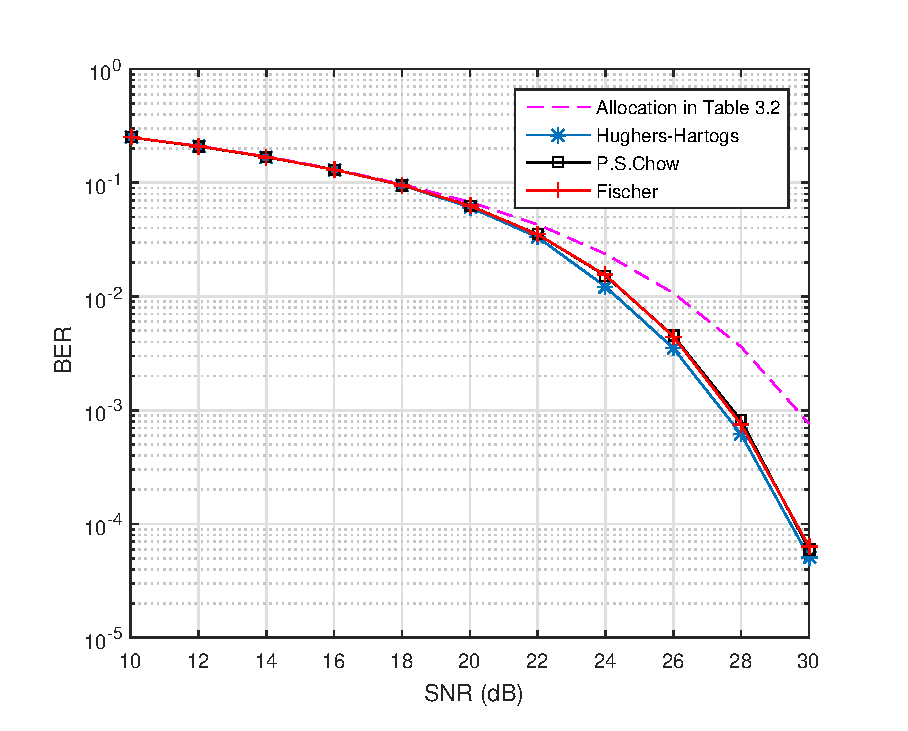
\includegraphics[width=0.9\textwidth]{figures/chapter-4/BERonDiffAlgo.eps}
\caption{SNR=25 dB时不同子载波上的误比特率}
\label{fig:berOnDiffAlgo}
\end{figure}

\begin{figure}[htbp]
\centering
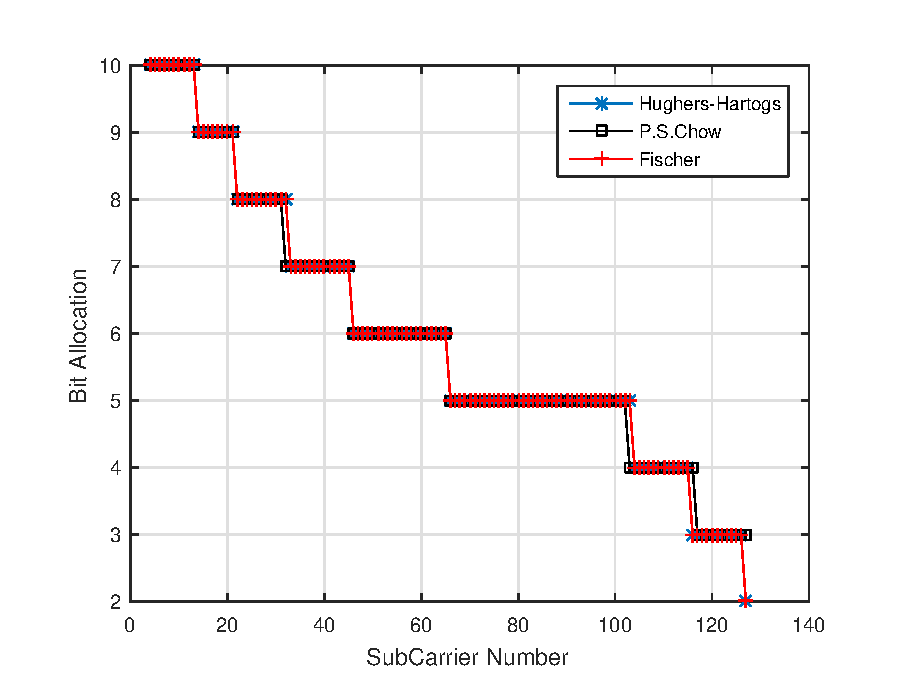
\includegraphics[width=0.9\textwidth]{figures/chapter-4/loadedBit.eps}
\caption{三种算法比特分配结果比较}
\label{fig:loadedBit}
\end{figure}

\begin{figure}[htbp]
\centering
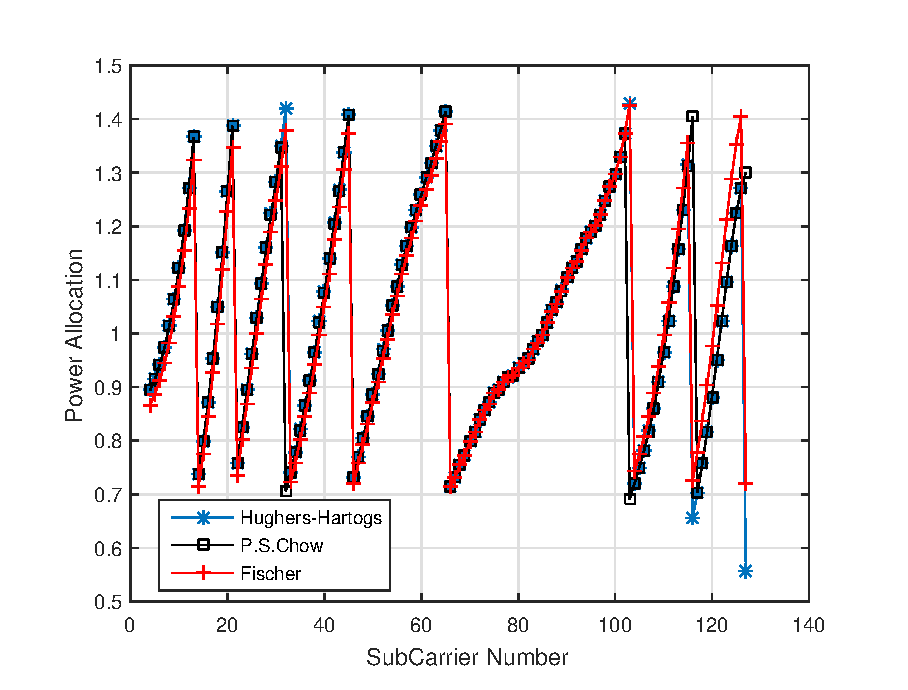
\includegraphics[width=0.9\textwidth]{figures/chapter-4/loadedPower.eps}
\caption{三种算法功率分配结果比较}
\label{fig:loadedPower}
\end{figure}

%\begin{figure}[htbp]
%    \centering
%    \subfloat[比特分配]{
%        \label{fig:Sim_Channel_time}
%        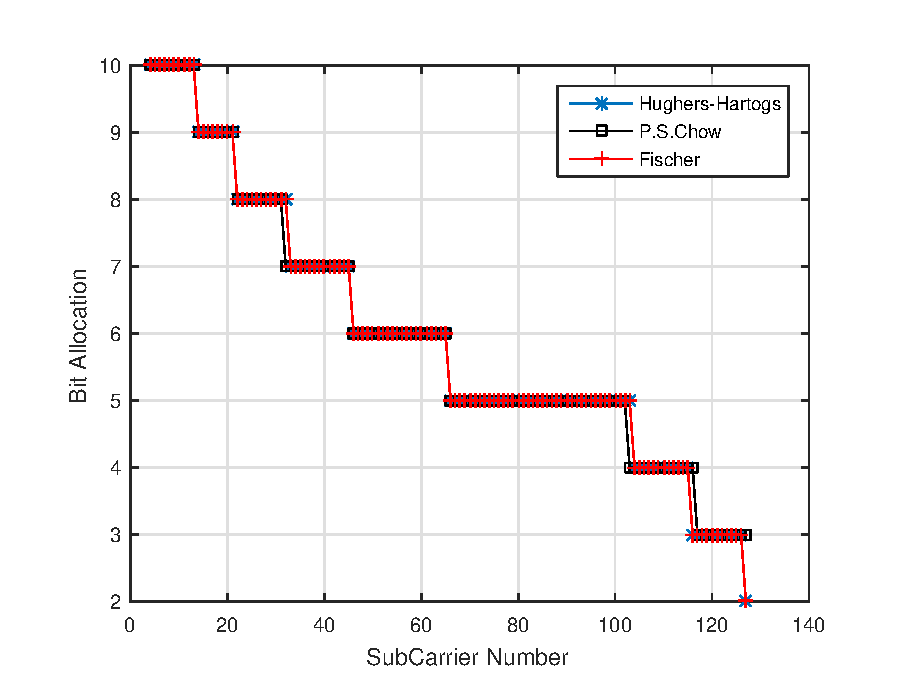
\includegraphics[width=0.5\textwidth]{figures/chapter-4/loadedBit.eps}
%    }
%    \subfloat[功率分配]{
%        \label{fig:Sim_Channel_frequency}
%        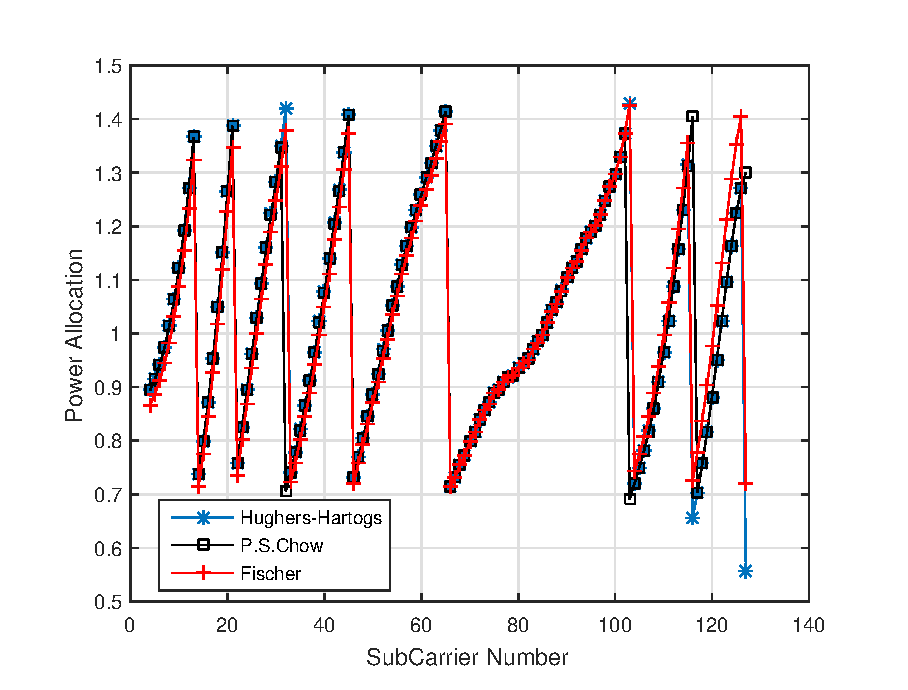
\includegraphics[width=0.5\textwidth]{figures/chapter-4/loadedPower.eps}
%    }
%    \caption{三种算法比特功率分配结果比较}
%    \label{fig:bitPowerAlloactionComparison}
%\end{figure}
\section{可见光通信中的自适应方案研究}
\section{本章小结}

